\documentclass[12pt]{article}
\usepackage[utf8]{inputenc}
\usepackage[T1]{fontenc}
\usepackage[english]{babel}
\usepackage{amsmath, amssymb, amsthm}
\usepackage{geometry}
\usepackage{titling}
\usepackage{fancyhdr}
\usepackage{lipsum}
\usepackage{parskip}
\usepackage{forest}
\usepackage{tikz}
\usepackage{stmaryrd}
\usepackage{listings}
\usepackage{graphicx}
\usepackage{float}
\usepackage{subcaption}
\usepackage{csvsimple}

\geometry{top=4cm, bottom=4cm, left=4cm, right=4cm}
\pagestyle{fancy}
\fancyhf{}
\rhead{Pierre Pili $\cdot$ Marie Gardie $\cdot$ Isée Biglietti}
\lhead{Macroeconomics 1}
\cfoot{\thepage}

\title{MACROECONOMICS 1 - HOMEWORK}
\author{PILI Pierre $\cdot$ GARDIE Marie $\cdot$ BIGLIETTI Isée}
\date{\today}
\begin{document}
\maketitle
\section{Data Work}
\subsubsection*{}
We used a data about France comming from the FRED website. To be able to respond to the questions of this exercise, we downloaded 6 different data: 
\begin{itemize}
    \item The Real Gross Domestic Product for France (CLVMNACSCAB1GQFR), in millions of 2010 euros
    \item The Private Final Consumption Expenditure for France (NAEXKP02FRQ189S), in euros
    \item The Gross Fixed Capital Formation for France (NAEXKP04FRQ189S), in euros
    \item The Average Annual Hours Worked by Persons Engaged for France (AVHWPEFRA065NRUG), in hours
    \item The Employment in France (FRAEMPT), in millions of people
    \item The total population for France (POPTOTFRA647NWDB), in persons
\end{itemize}
After some conversions, we use the Total population data to make Private Final Consumption and Gross fixed capital formation per capita.
We used Employment data as well as Average Annual Hours Worked by Persons Engaged and Total population to obtain per capita Hours Worked. 
Therefore, we easily obtain a joint dataframe with our 5 variables of ineterest: Year, and Investment, Consumption, Hours Worked and GDP, all per capita.

\begin{figure}
    \centering
  
    \begin{subfigure}[b]{0.45\textwidth}
      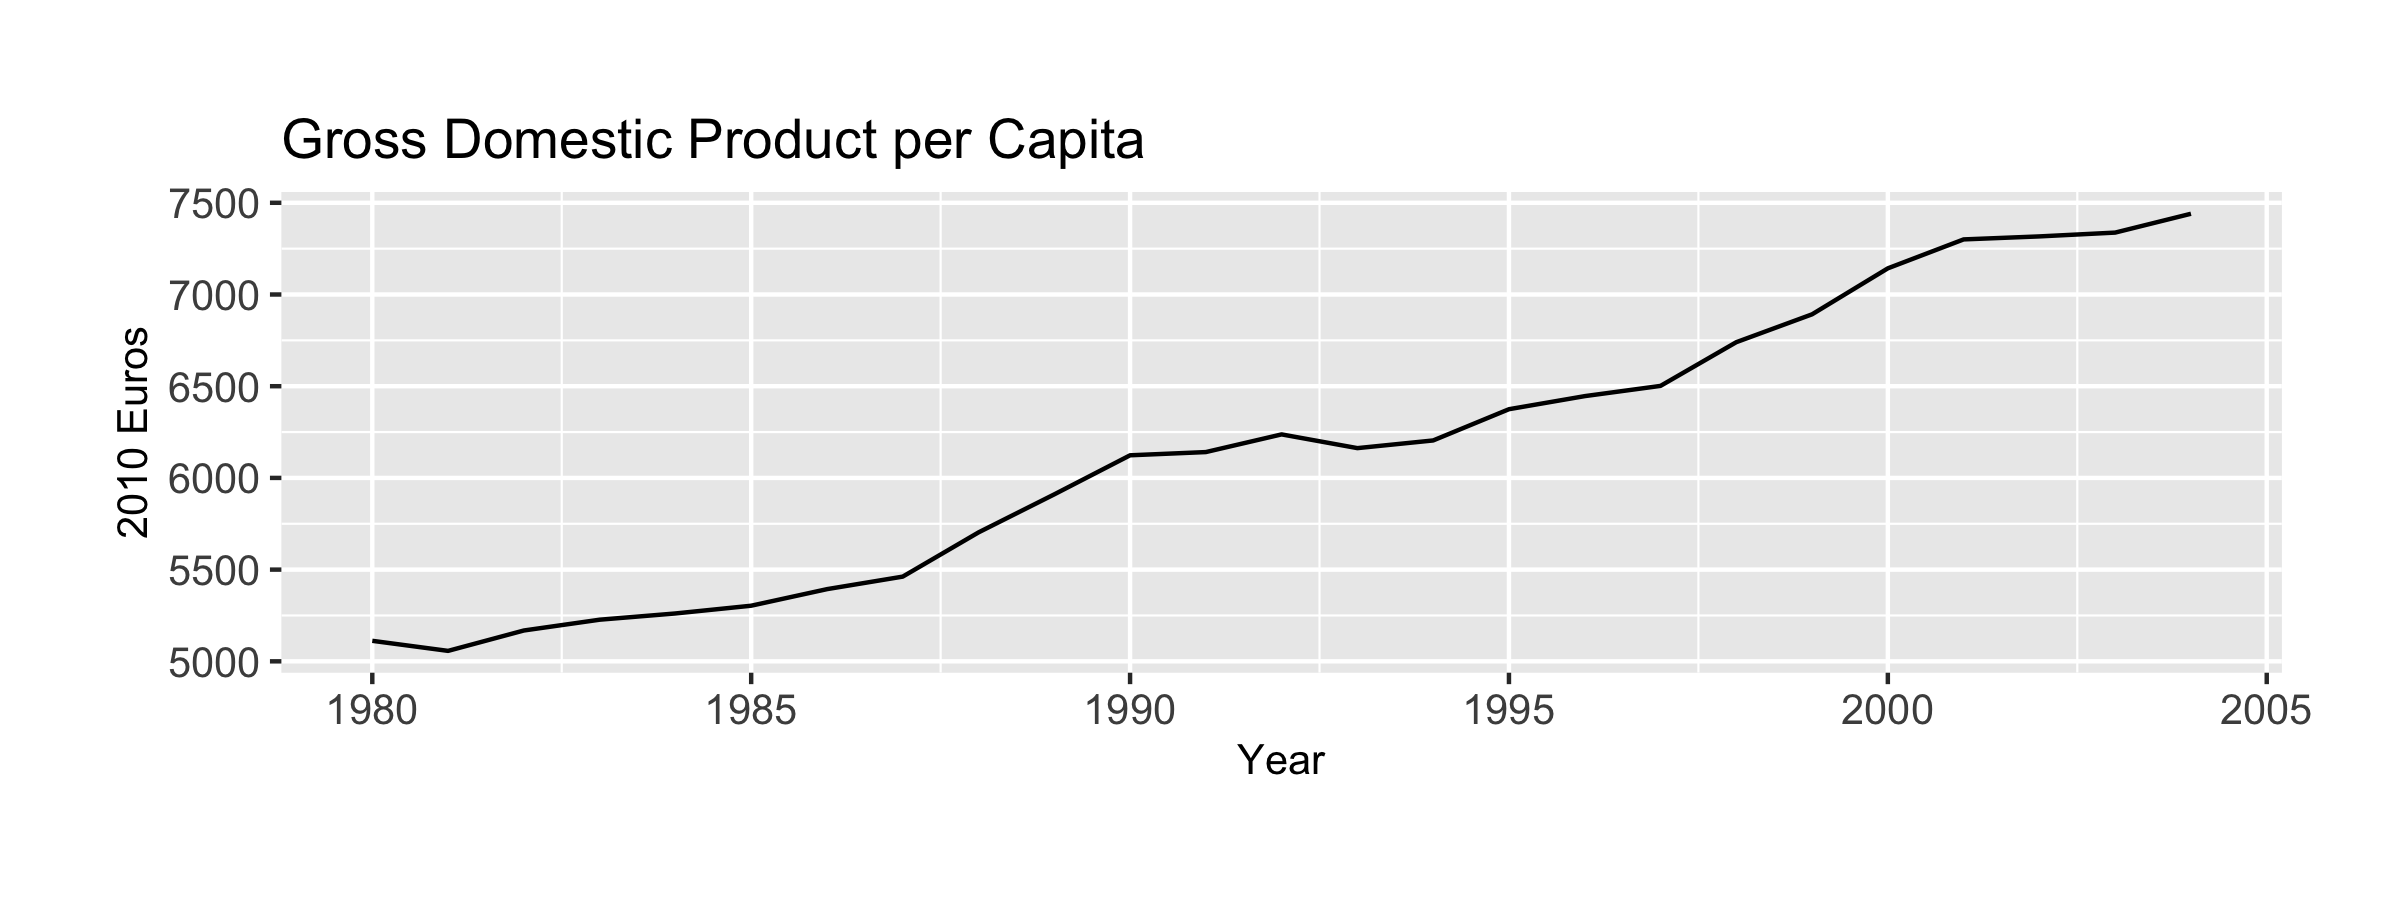
\includegraphics[width=\textwidth]{OUTPUT/MEDIA/gdp_pc.png}
      \caption{GDP}
    \end{subfigure}
    \hfill
    \begin{subfigure}[b]{0.45\textwidth}
      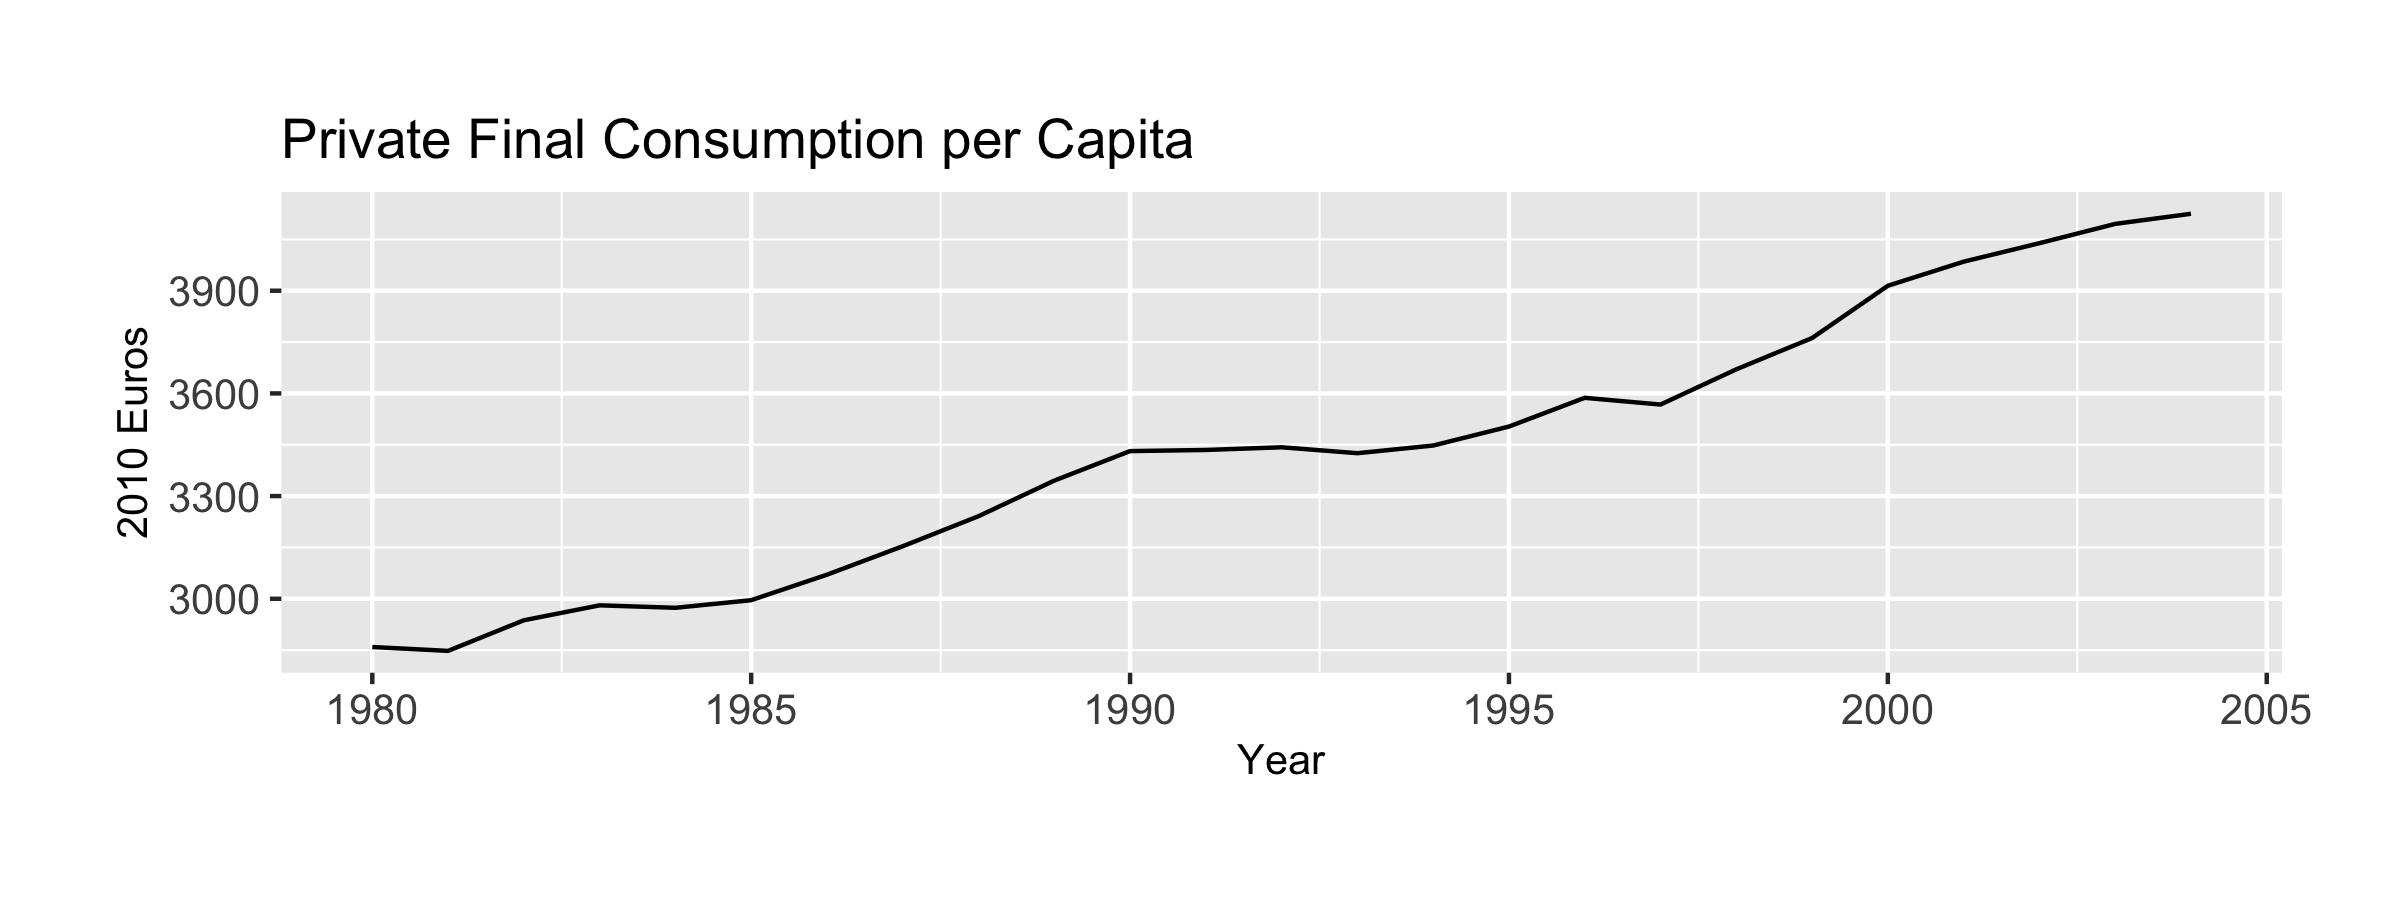
\includegraphics[width=\textwidth]{OUTPUT/MEDIA/cons_pc.png}
      \caption{Consumption}
    \end{subfigure}
  
    \vspace{\baselineskip} % Ajouter un espace vertical
  
    \begin{subfigure}[b]{0.45\textwidth}
      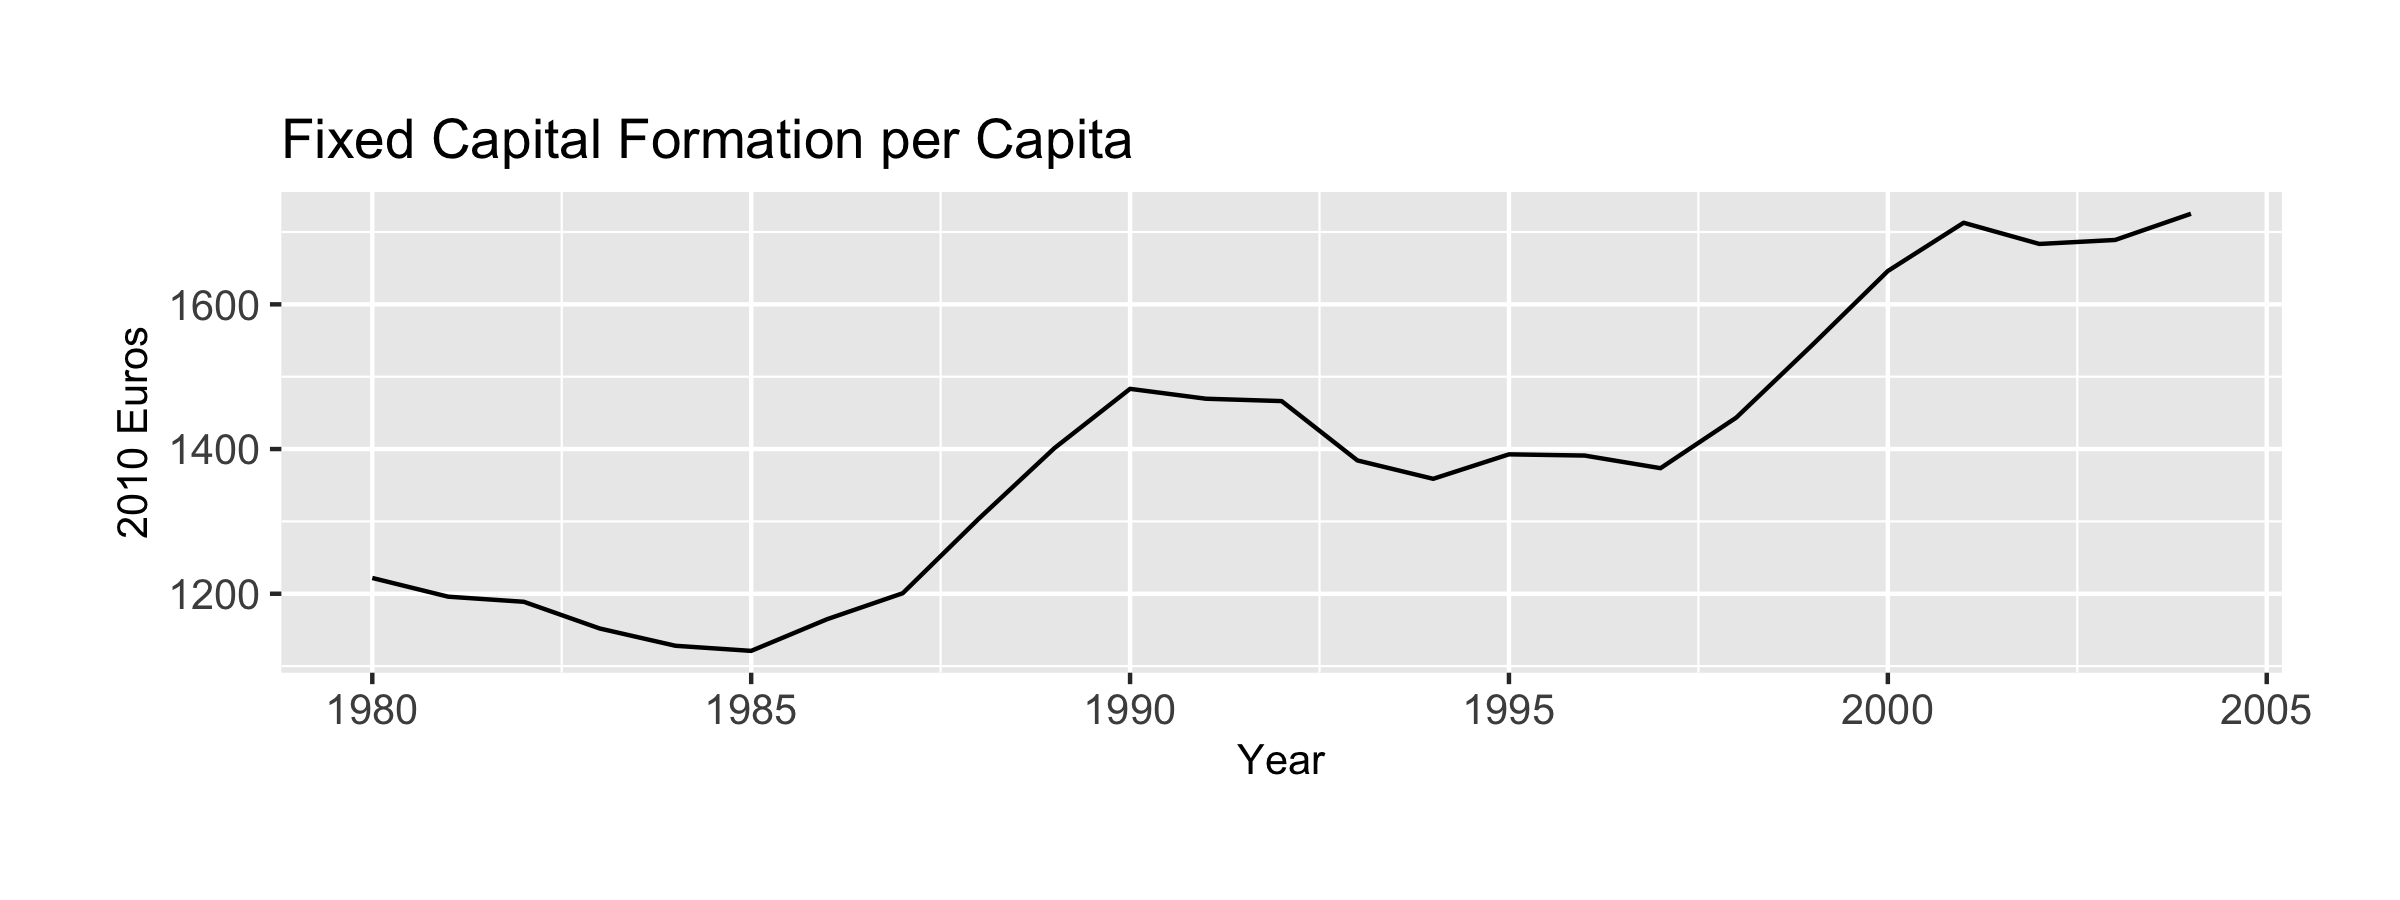
\includegraphics[width=\textwidth]{OUTPUT/MEDIA/inv_pc.png}
      \caption{Investment}
    \end{subfigure}
    \hfill
    \begin{subfigure}[b]{0.45\textwidth}
      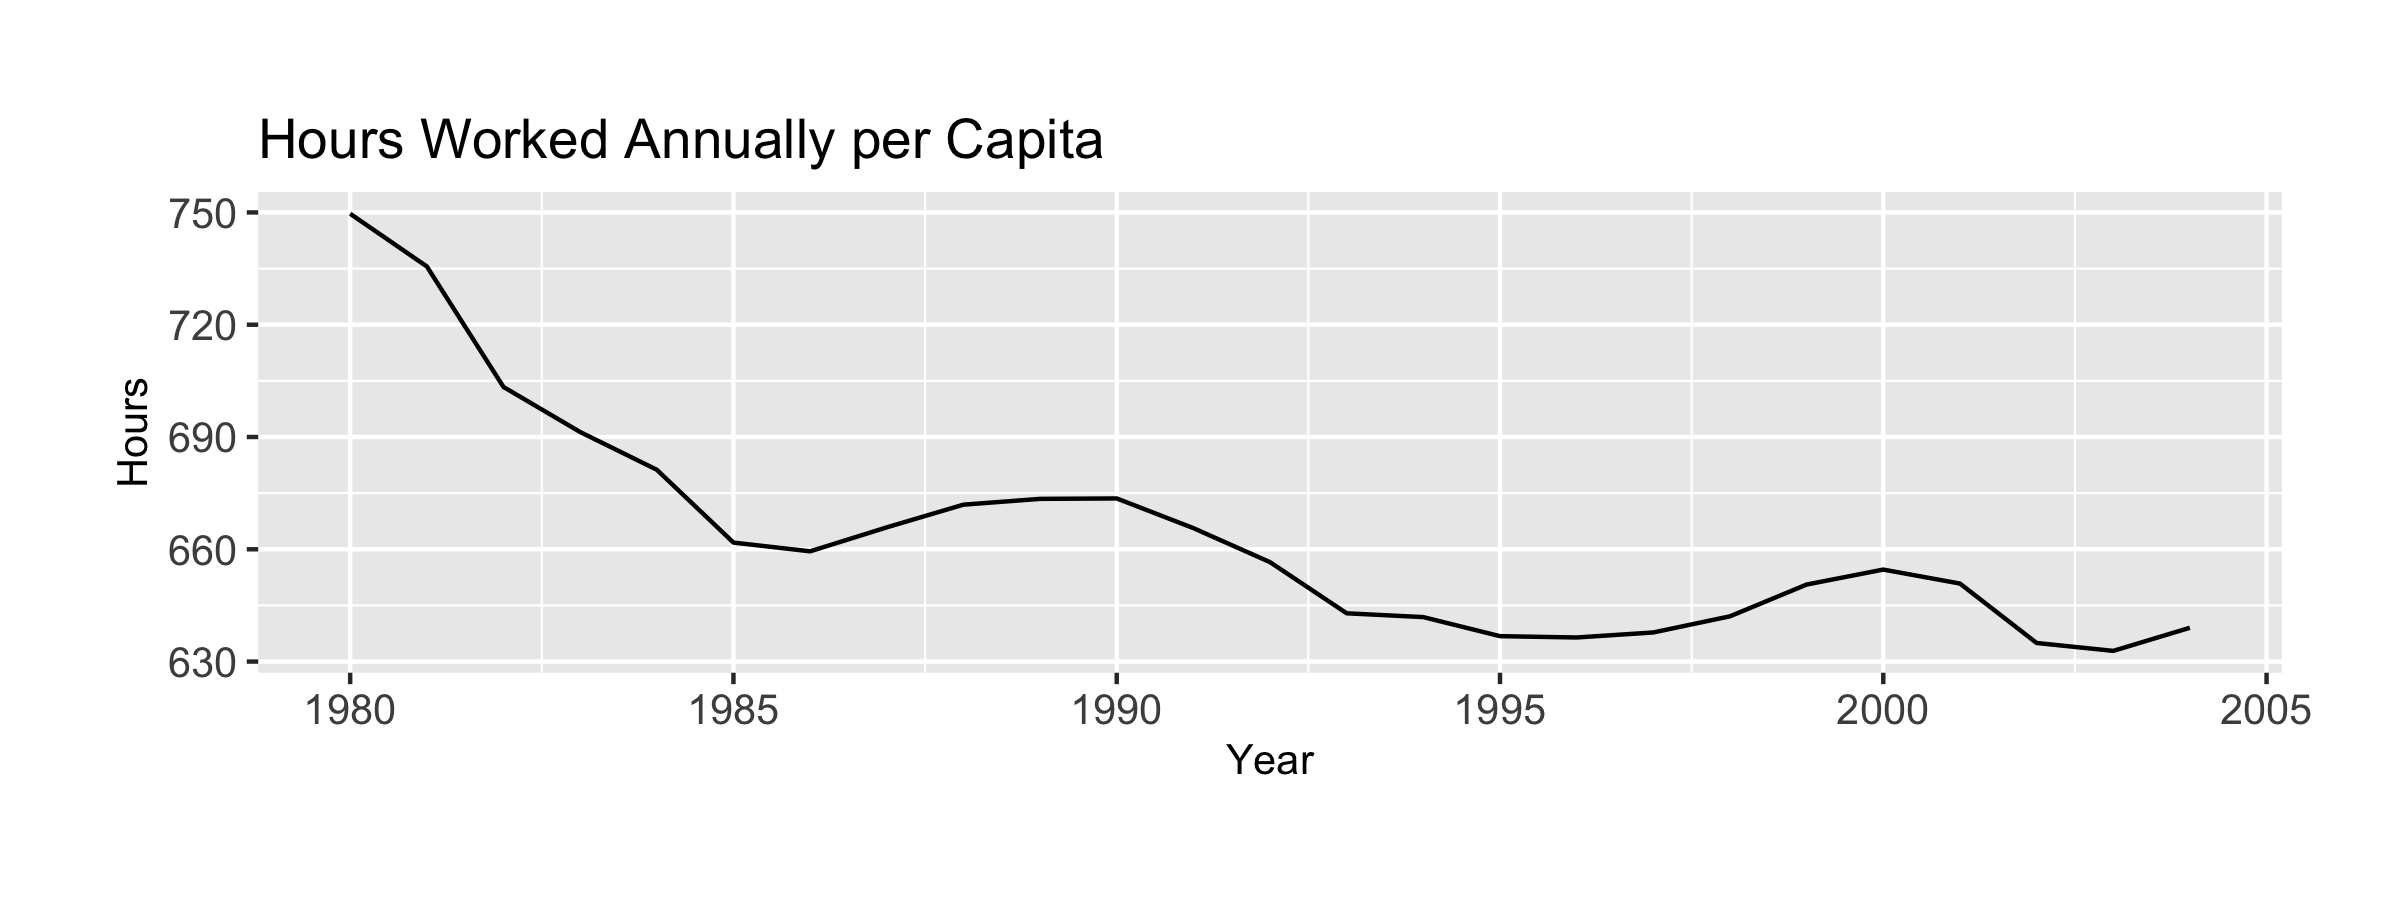
\includegraphics[width=\textwidth]{OUTPUT/MEDIA/hours_pc.png}
      \caption{Hours worked}
    \end{subfigure}
  
    \caption{Descriptive trend of our raw data}
    \label{fig:descriptive}
  \end{figure}

\ref{fig:descriptive} show some descriptive statistics about how our raw variables of interest behave. 
We observe cycles and trends on these graphs. One can estimate a linear trend for the logarithms of the four data series obtaining table 1:



\subcaptionbox{Tableau 1\label{tab:sub1}}[0.45\textwidth][c]{%
\begin{tabular}{ccc}
  \toprule
  Colonne 1 & Colonne 2 & Colonne 3 \\
  \midrule
  Donnée 1 & Donnée 2 & Donnée 3 \\
  Donnée 4 & Donnée 5 & Donnée 6 \\
  \bottomrule
\end{tabular}%
}




\begin{figure}
    \centering
    \subcaptionbox{lm GDP}[0.45\textwidth][c]{%
      \centering
      \caption{Real Gross Domestic Product in 2010 Euros per Capita With Respect to Time} 
      % GDP
      \begin{tabular}{@{\extracolsep{5pt}}lD{.}{.}{-3} } 
        \\[-1.8ex]\hline 
        \hline \\[-1.8ex] 
         & \multicolumn{1}{c}{\textit{Dependent variable:}} \\ 
        \cline{2-2} 
        \\[-1.8ex] & \multicolumn{1}{c}{log(GDP)} \\ 
        \hline \\[-1.8ex] 
         YEAR & 0.017^{***} \\ 
          & (0.001) \\ 
          & \\ 
         Constant & -25.479^{***} \\ 
          & (1.002) \\ 
          & \\ 
        \hline \\[-1.8ex] 
        Observations & \multicolumn{1}{c}{25} \\ 
        R$^{2}$ & \multicolumn{1}{c}{0.981} \\ 
        Adjusted R$^{2}$ & \multicolumn{1}{c}{0.980} \\ 
        Residual Std. Error & \multicolumn{1}{c}{0.018 (df = 23)} \\ 
        F Statistic & \multicolumn{1}{c}{1,163.722$^{***}$ (df = 1; 23)} \\ 
        \hline 
        \hline \\[-1.8ex] 
        \textit{Note:}  & \multicolumn{1}{r}{$^{*}$p$<$0.1; $^{**}$p$<$0.05; $^{***}$p$<$0.01} \\
        \end{tabular}
    }
    \hfill
    \subcaptionbox{lm Consumption}[0.45\textwidth][c]{%
      \centering
      \caption{Gross Fixed Capital Formation in Constant Prices per Capita With Respect to Time} 
      % Consumption
      \begin{tabular}{@{\extracolsep{5pt}}lD{.}{.}{-3} } 
        \\[-1.8ex]\hline 
        \hline \\[-1.8ex] 
         & \multicolumn{1}{c}{\textit{Dependent variable:}} \\ 
        \cline{2-2} 
        \\[-1.8ex] & \multicolumn{1}{c}{log(CONSUMPTION)} \\ 
        \hline \\[-1.8ex] 
         YEAR & 0.016^{***} \\ 
          & (0.0005) \\ 
          & \\ 
         Constant & -22.854^{***} \\ 
          & (0.982) \\ 
          & \\ 
        \hline \\[-1.8ex] 
        Observations & \multicolumn{1}{c}{25} \\ 
        R$^{2}$ & \multicolumn{1}{c}{0.977} \\ 
        Adjusted R$^{2}$ & \multicolumn{1}{c}{0.976} \\ 
        Residual Std. Error & \multicolumn{1}{c}{0.018 (df = 23)} \\ 
        F Statistic & \multicolumn{1}{c}{996.105$^{***}$ (df = 1; 23)} \\ 
        \hline 
        \hline \\[-1.8ex] 
        \textit{Note:}  & \multicolumn{1}{r}{$^{*}$p$<$0.1; $^{**}$p$<$0.05; $^{***}$p$<$0.01} \\ 
        \end{tabular} 
    }
    \vspace{\baselineskip} % Ajouter un espace vertical
    \subcaptionbox{lm Investment}[0.45\textwidth][c]{%
      \centering
      \caption{Private Final Consumption Expenditure in Constant Prices per Capita With Respect to Time} 
      % investment
      \begin{tabular}{@{\extracolsep{5pt}}lD{.}{.}{-3} } 
        \\[-1.8ex]\hline 
        \hline \\[-1.8ex] 
         & \multicolumn{1}{c}{\textit{Dependent variable:}} \\ 
        \cline{2-2} 
        \\[-1.8ex] & \multicolumn{1}{c}{log(INVESTMENT)} \\ 
        \hline \\[-1.8ex] 
         YEAR & 0.017^{***} \\ 
          & (0.002) \\ 
          & \\ 
         Constant & -26.808^{***} \\ 
          & (3.294) \\ 
          & \\ 
        \hline \\[-1.8ex] 
        Observations & \multicolumn{1}{c}{25} \\ 
        R$^{2}$ & \multicolumn{1}{c}{0.823} \\ 
        Adjusted R$^{2}$ & \multicolumn{1}{c}{0.815} \\ 
        Residual Std. Error & \multicolumn{1}{c}{0.060 (df = 23)} \\ 
        F Statistic & \multicolumn{1}{c}{106.798$^{***}$ (df = 1; 23)} \\ 
        \hline 
        \hline \\[-1.8ex] 
        \textit{Note:}  & \multicolumn{1}{r}{$^{*}$p$<$0.1; $^{**}$p$<$0.05; $^{***}$p$<$0.01} \\ 
        \end{tabular}
    }
    \hfill
    \subcaptionbox{lm Hours worked}[0.45\textwidth][c]{%
      \centering
      \caption{Hours Worked Annualy per Capita With Respect to Time} 
      % Hours
      \begin{tabular}{@{\extracolsep{5pt}}lD{.}{.}{-3} } 
        \\[-1.8ex]\hline 
        \hline \\[-1.8ex] 
         & \multicolumn{1}{c}{\textit{Dependent variable:}} \\ 
        \cline{2-2} 
        \\[-1.8ex] & \multicolumn{1}{c}{log(HOURS\_WORKED)} \\ 
        \hline \\[-1.8ex] 
         YEAR & -0.005^{***} \\ 
          & (0.001) \\ 
          & \\ 
         Constant & 16.407^{***} \\ 
          & (1.392) \\ 
          & \\ 
        \hline \\[-1.8ex] 
        Observations & \multicolumn{1}{c}{25} \\ 
        R$^{2}$ & \multicolumn{1}{c}{0.688} \\ 
        Adjusted R$^{2}$ & \multicolumn{1}{c}{0.674} \\ 
        Residual Std. Error & \multicolumn{1}{c}{0.025 (df = 23)} \\ 
        F Statistic & \multicolumn{1}{c}{50.698$^{***}$ (df = 1; 23)} \\ 
        \hline 
        \hline \\[-1.8ex] 
        \textit{Note:}  & \multicolumn{1}{r}{$^{*}$p$<$0.1; $^{**}$p$<$0.05; $^{***}$p$<$0.01} \\ 
        \end{tabular} 
    }
    \caption{Four regression tables from our four variables' trend}
    \label{fig:lmtables}
\end{figure}

These table can be illustrated as follow:

\begin{figure}
    \centering
    \begin{subfigure}[b]{0.45\textwidth}
      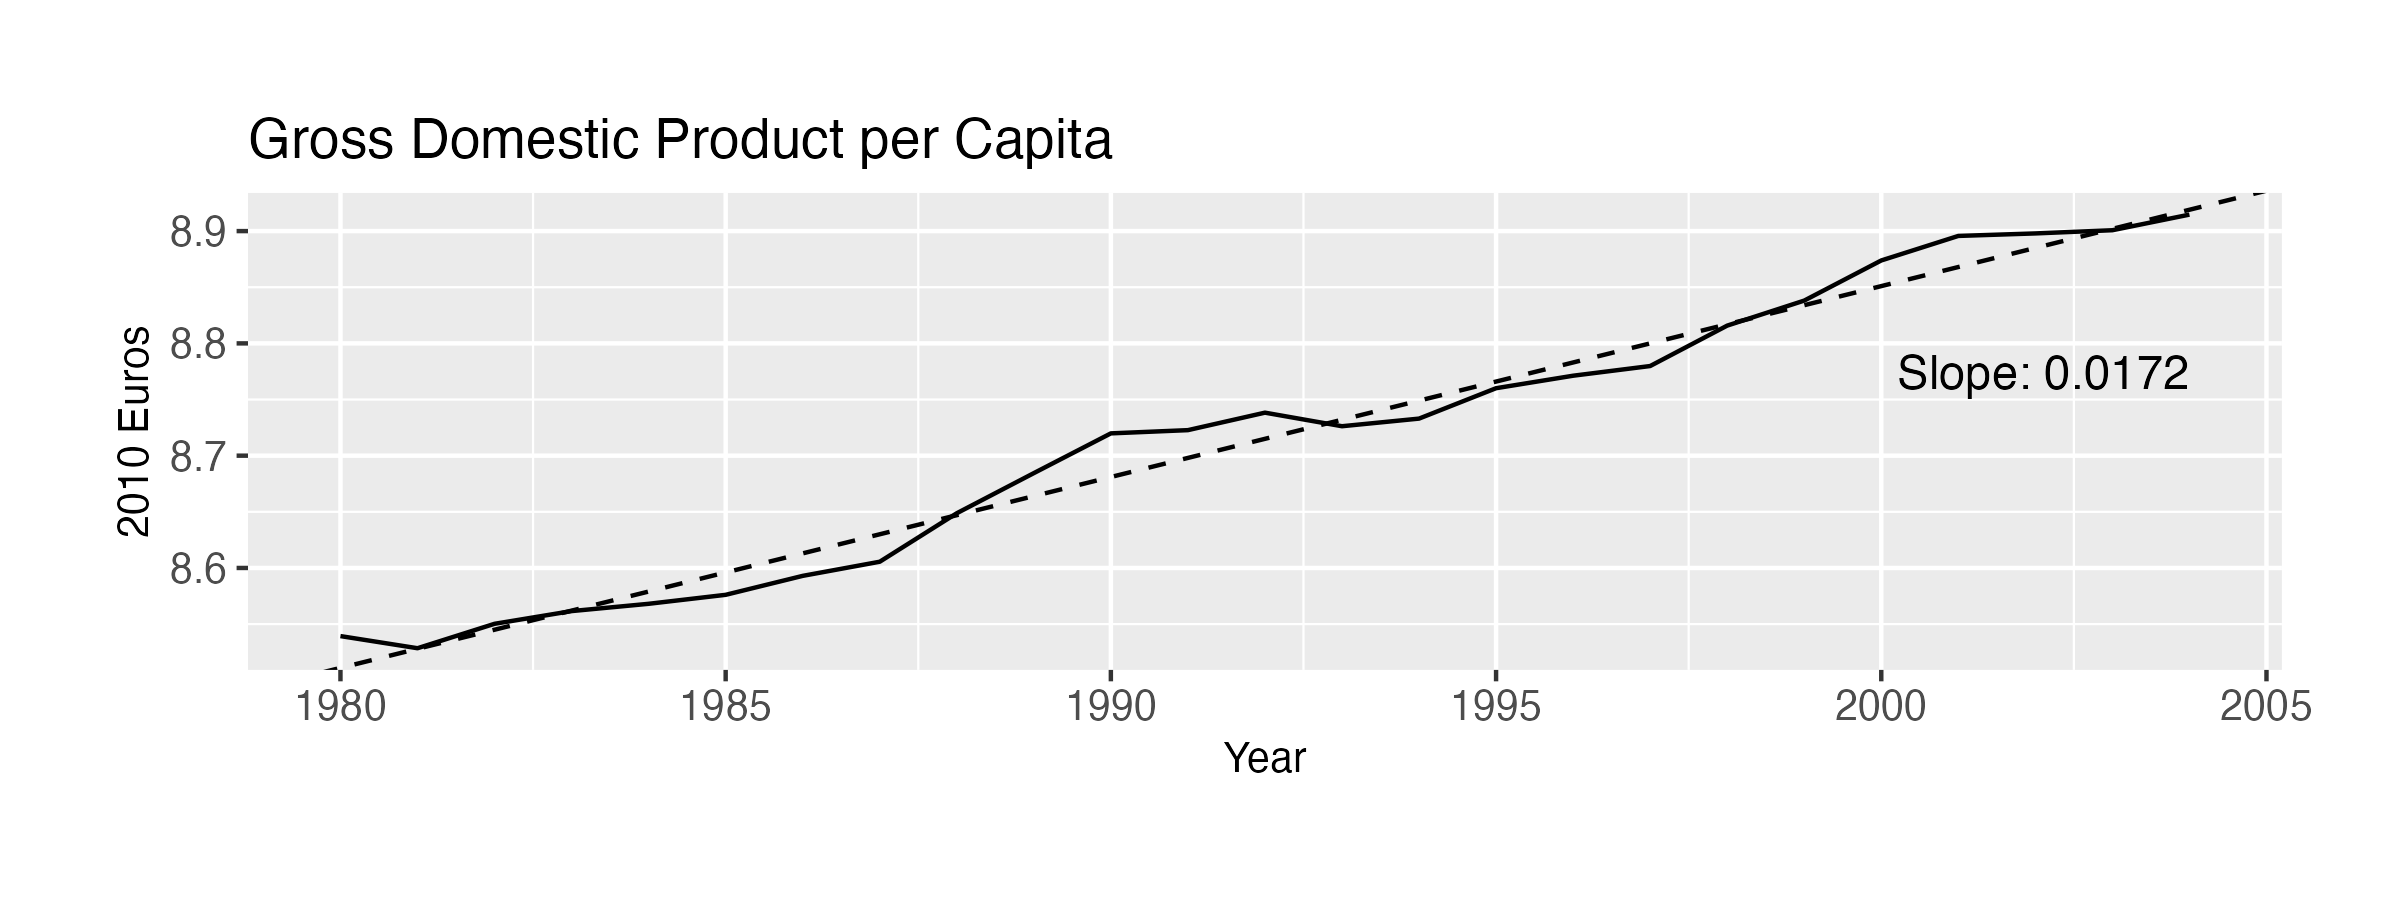
\includegraphics[width=\textwidth]{OUTPUT/MEDIA/loggdp_pc.png}
      \caption{Log GDP}
    \end{subfigure}
    \hfill
    \begin{subfigure}[b]{0.45\textwidth}
      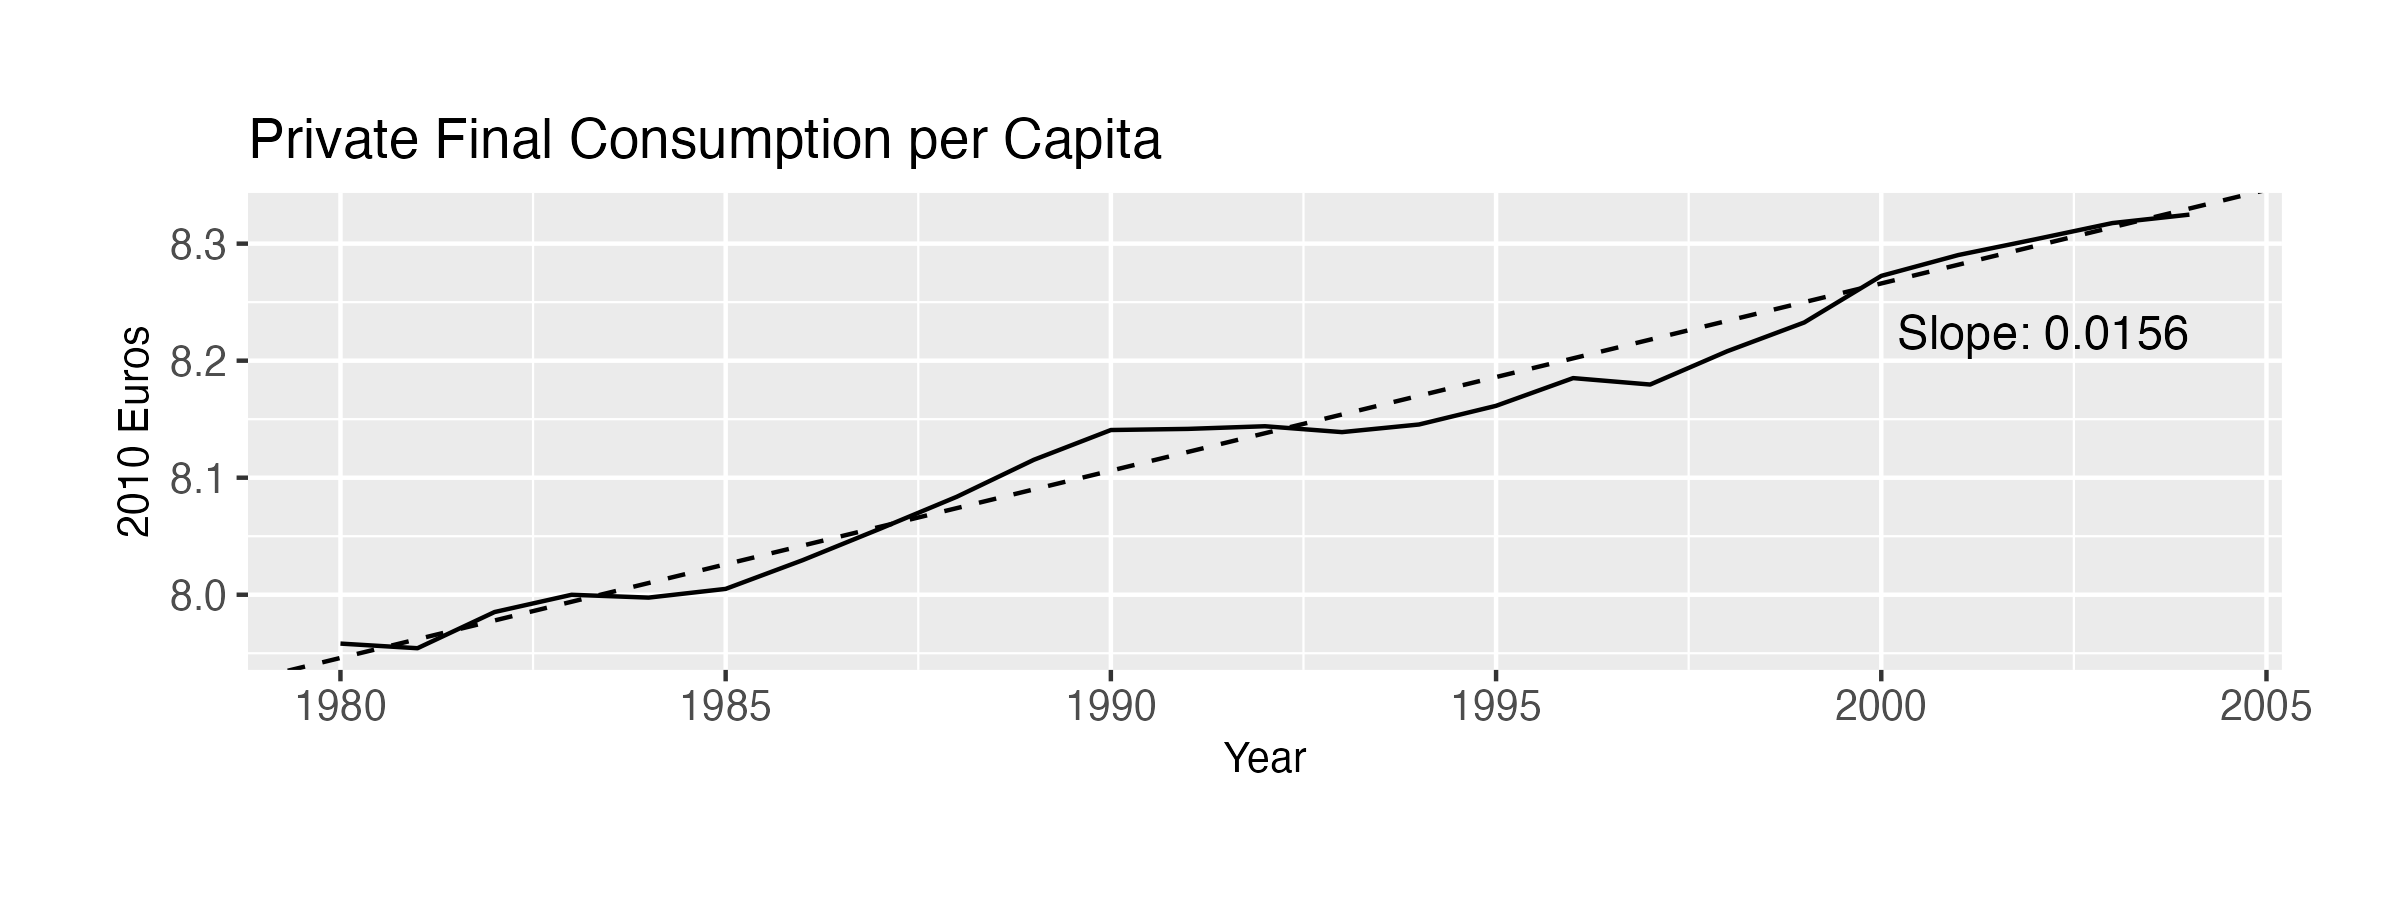
\includegraphics[width=\textwidth]{OUTPUT/MEDIA/logcons_pc.png}
      \caption{Log Consumption}
    \end{subfigure}
    \vspace{\baselineskip} % Ajouter un espace vertical
    \begin{subfigure}[b]{0.45\textwidth}
      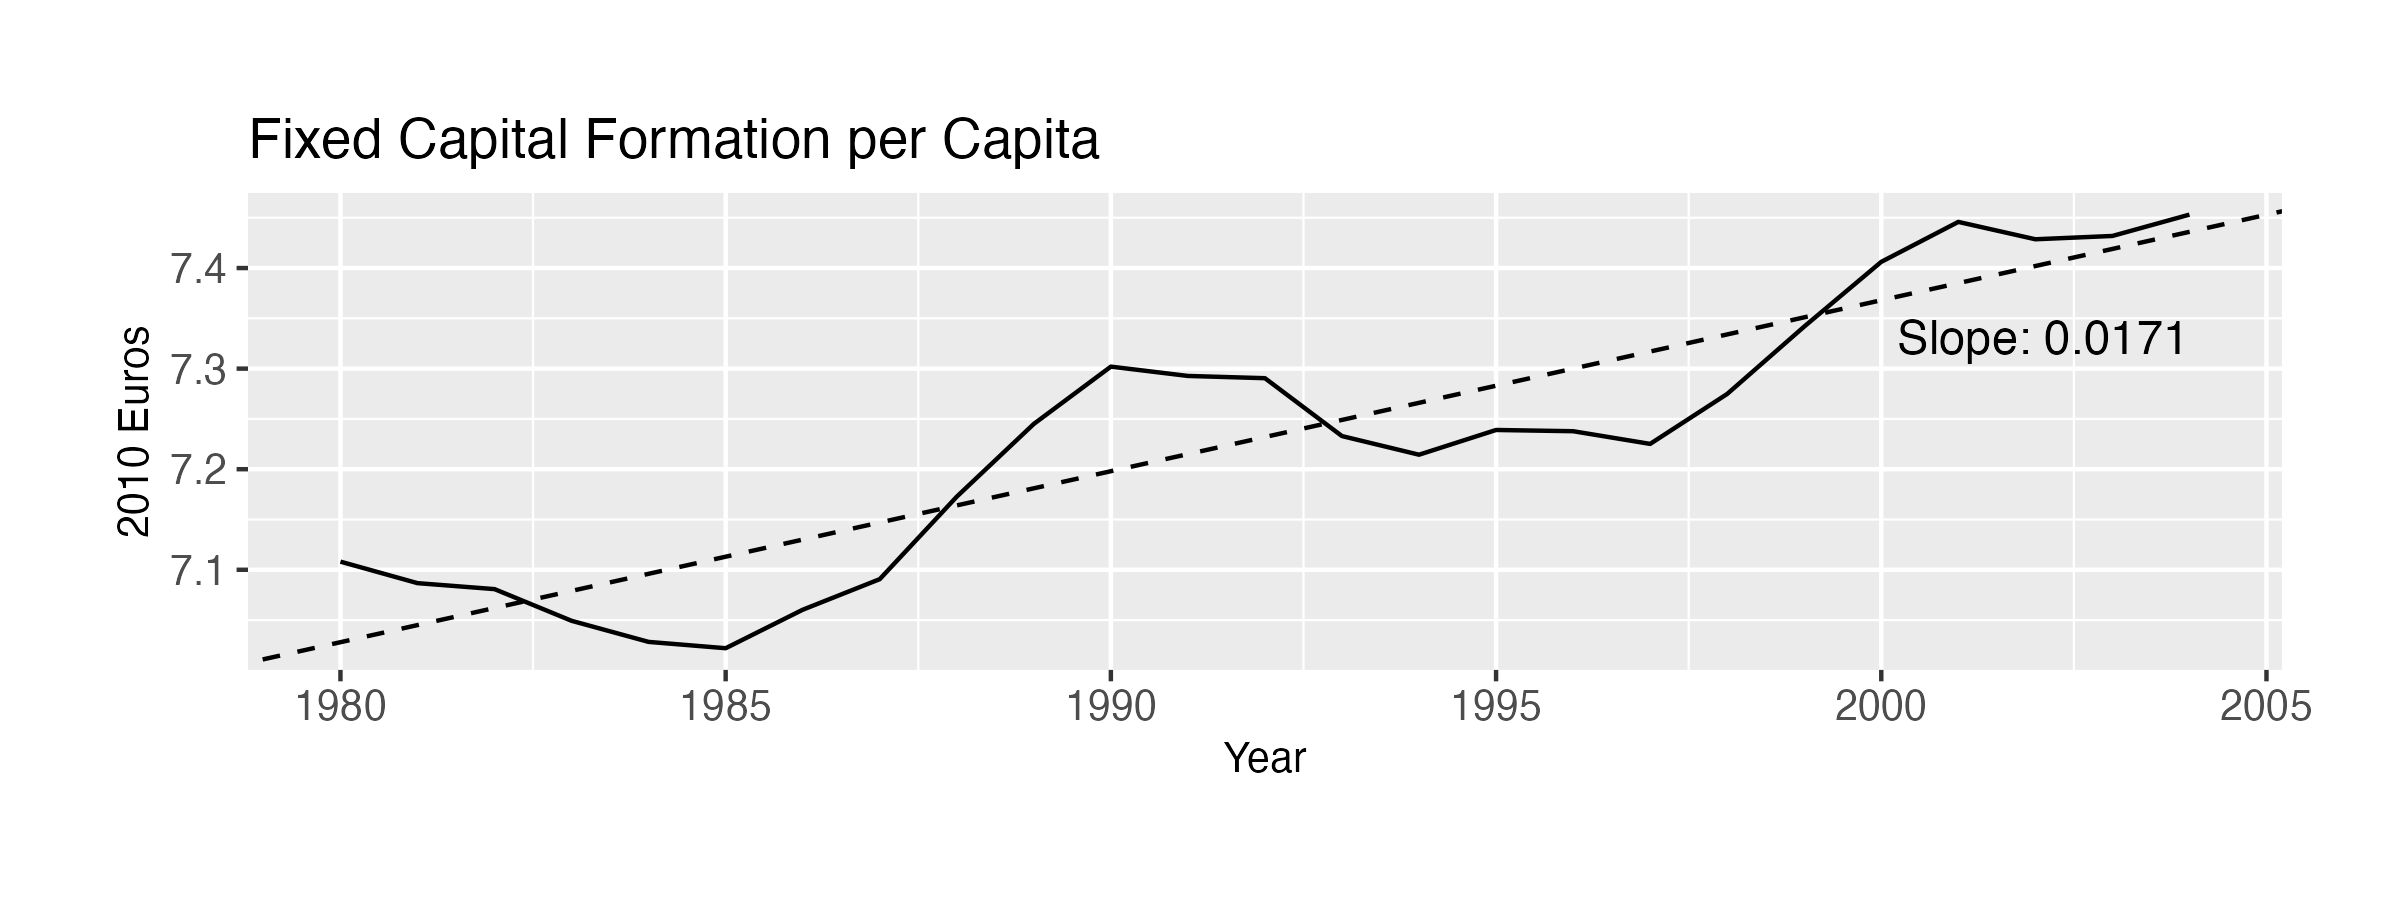
\includegraphics[width=\textwidth]{OUTPUT/MEDIA/loginv_pc.png}
      \caption{Log Investment}
    \end{subfigure}
    \hfill
    \begin{subfigure}[b]{0.45\textwidth}
      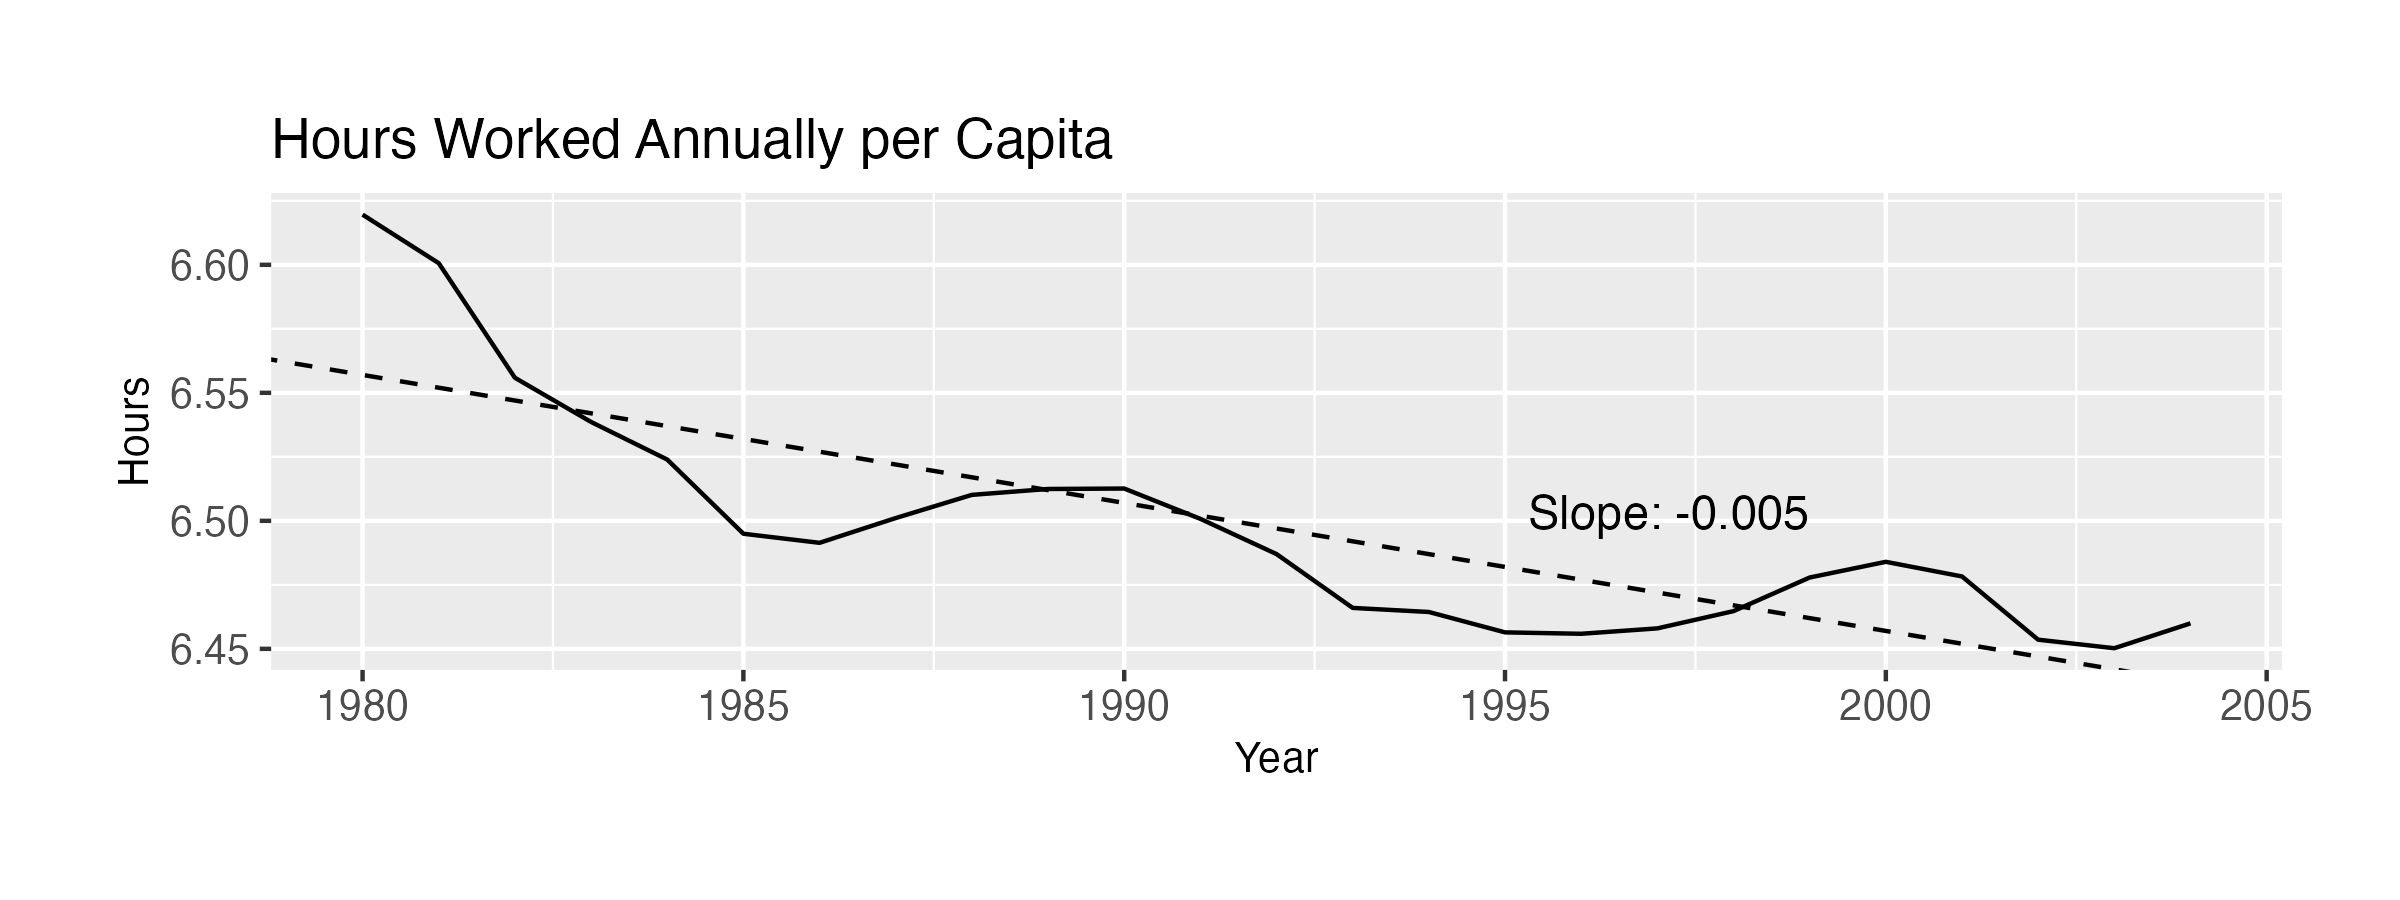
\includegraphics[width=\textwidth]{OUTPUT/MEDIA/loghours_pc.png}
      \caption{Log Hours worked}
    \end{subfigure}
    \caption{Linear trend for the logarithms of our four data series}
    \label{fig:logtrends}
\end{figure}

The trend is there represented by the linear relation, a trend with constant growth rate, were any deviation from this trend, represented by the dashed line on \ref{fig:logtrends} are what we can call "Business Cycles".
But we would like to visualize better those business cycles. Using a HP-filter, we can decompose the trending and the cyclical part from the variations of each variables through time. \ref{fig:cycles} shows us that our 4 variables seems to vary jointly through time, to be procyclical. However, some are still wider than others. 

\begin{figure}[h]
    \centering
    \begin{tikzpicture}[baseline=(current bounding box.center)]
        \node at (0,0) {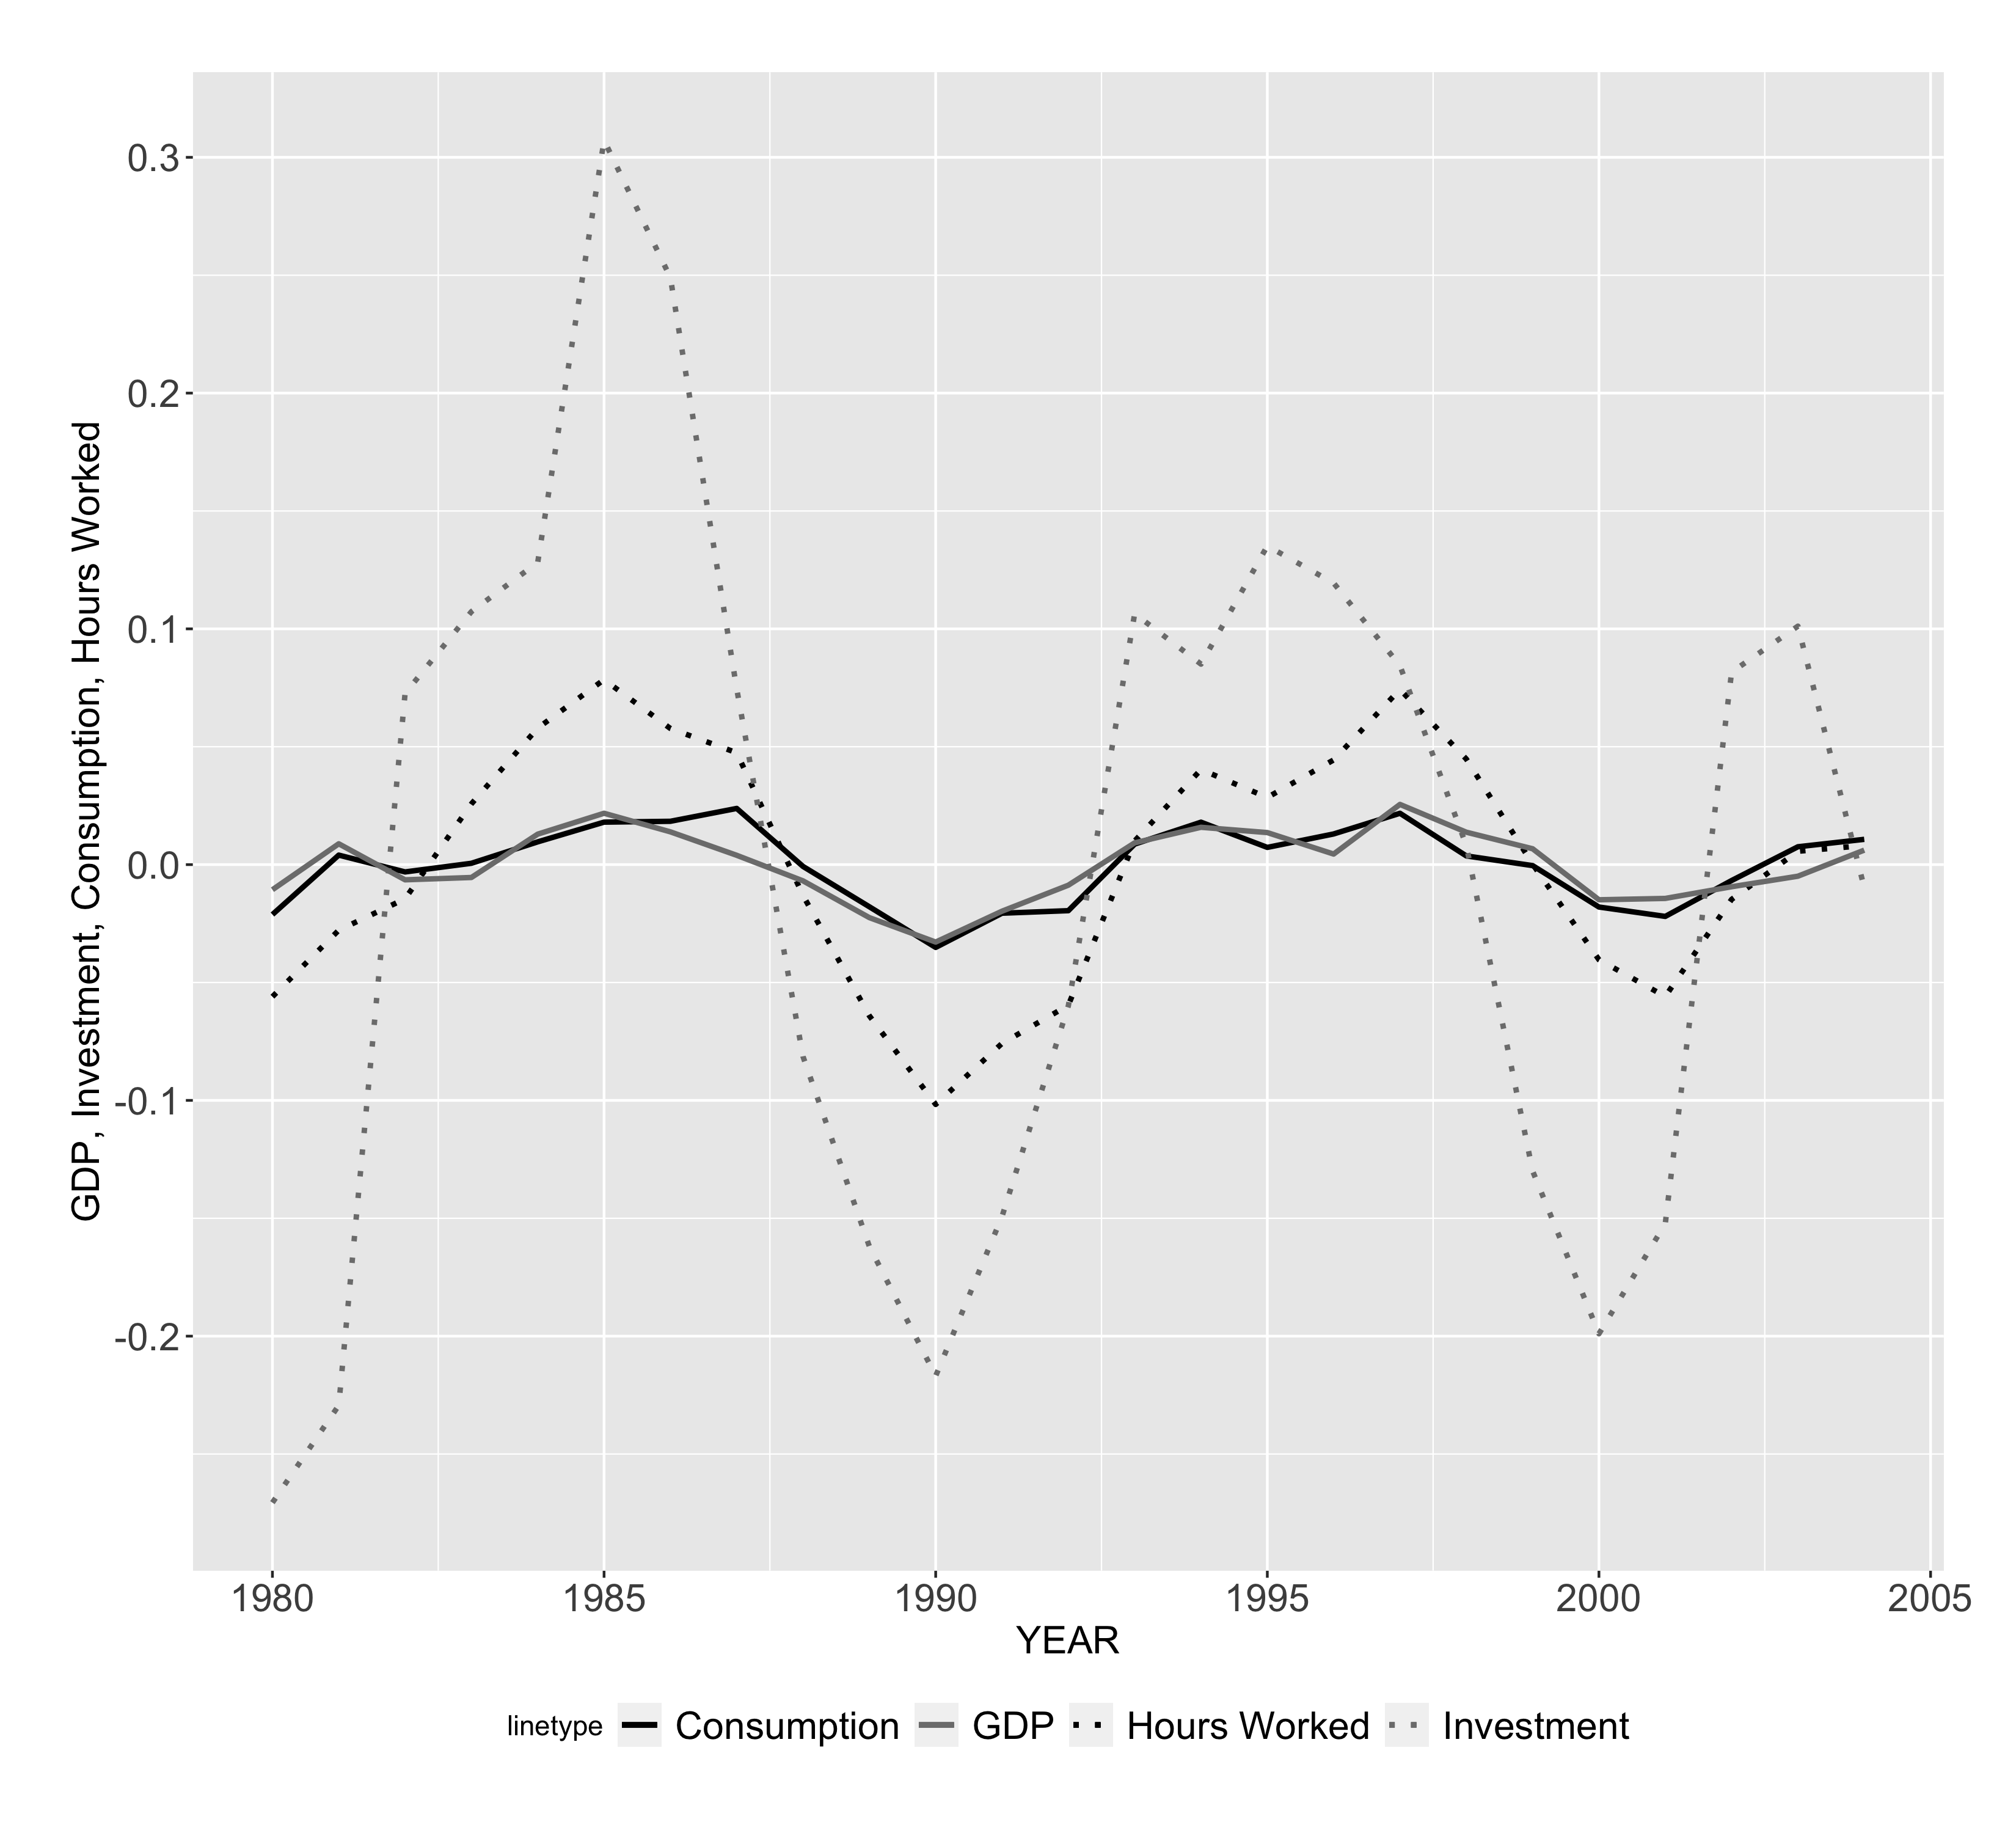
\includegraphics[width=0.9\textwidth]{OUTPUT/MEDIA/cycles.png}};
    \end{tikzpicture}
    \caption{Business Cycles in our main variables' vraiations}
    \label{fig:cycles}
\end{figure}

Those illustrations and tables help us better understand the compositions of these main macroeconomic variables' variations trough time. 
The graph clearly shows the ascending and descending periods of the cycles, as well as the fact that certain variables, such as GDP and hours worked, have more stable, less wide-ranging oscillations than the other two (consumption and investment).
While it gives us an idea of our variables' behavior, though, it doesn't allow us to compare them with precision. 

\subsubsection*{}
In order to compare variations of our variables of interest, we need to compute some indicators. 
In \ref{fig:corr_RSD}, one can observe the the relative standard deviations and correlation coefficients, taking GDP as a benchmark.

\begin{table}
    \centering
    \caption{Correlation coefficient and Relative Standard Deviations (RDS), with GDP as a benchmark}
    \label{tab:corr_RSD}
    \csvautotabular{OUTPUT/TABLES/corr_RSD.csv}
\end{table}

In the lecture, we evaluated the same indicators but for the case of the US. Let's compare our results to those. 
\newline
First of all, we had that consumption, investment and hours worked were strongly procyclical for the US. 
Observing that all of our correlation coeficient with GDP are positives and close to $1$, we can enforce the same conclusion for these $3$ variables, with consumption and investment being even more procyclical, their correlation coefficient being over $0.9$. 
\newline    
Second of all, we saw that for the US, consumption were less volatile than GDP, whereas investment were more.
Using the results we found for Relative Standard Deviation (RSD), we have that $\sigma_Y > \sigma_I > \sigma_C > \sigma_H$ for France. these differences make sense: they can be explained by the fact that we're not dealing with the same country, and so its political behaviour (investment, work and consumption) can be very different.

\end{document}



